\chapter{Introduction}
Matchmaking Encryption is a new form of encryption introduced by Ateniese et al. \cite{Ateniese} as a generalization of Attribute-Based Encryption (see \ref{sec:abe}) which enables several new applications where involved participants can specify fine-grained access policies to encrypted data, opening up new ways for secret communications.
\newline\newline
ME can be extremely useful in order to avoid liability or inappropriateness; indeed, some of the killer applications of ME are:
\begin{itemize}
    \item social matchmaking
    \item encrypting bids and votes
    \item censorship-resistant communication for marginalized communities in authoritarian countries.
\end{itemize}
In particular, in this context we consider two parties: the sender S with attributes $\sigma$ and the receiver R with attributes $\rho$.
They can both specify policies (i.e. access rights expressed in terms of attributes) the other party must satisfy in order for the message to be revealed.
The policies are represented as circuits $\mathbb{C} : \{0, 1\}^* \to \{0, 1\}$, while the attributes are binary strings of arbitrary length.
For instance, in the social matchmaking setting, S can encrypt a message $m$ containing his personal details and specify a policy $\mathbb{R}$ so that the message can be decrypted only by his ideal partner, i.e. one who matches the policy.
On the other end, R will be able to decrypt the message only if S corresponds to his ideal partner: this is again expressed through a policy $\mathbb{S}$. The decryption is successful if $\mathbb{S}(\sigma) = \mathbb{R}(\rho) = 1$, i.e. both the policies are matched.
\newline\newline
In Matchmaking Encryption, a trusted authority generates encryption and decryption keys associated, respectively, to attributes of the sender and the receiver.
The authority also generates an additional decryption key for the receiver, associated to an arbitrary policy of its choice.
The sender of the message can specify on the fly an arbitrary policy the receiver must satisfy in order for the message to be revealed.
The guarantee is now that the receiver will obtain the message if and only if a match occurs.
An example is given in figure \ref{fig:me_example}.
\begin{figure}[ht]
    \centering
    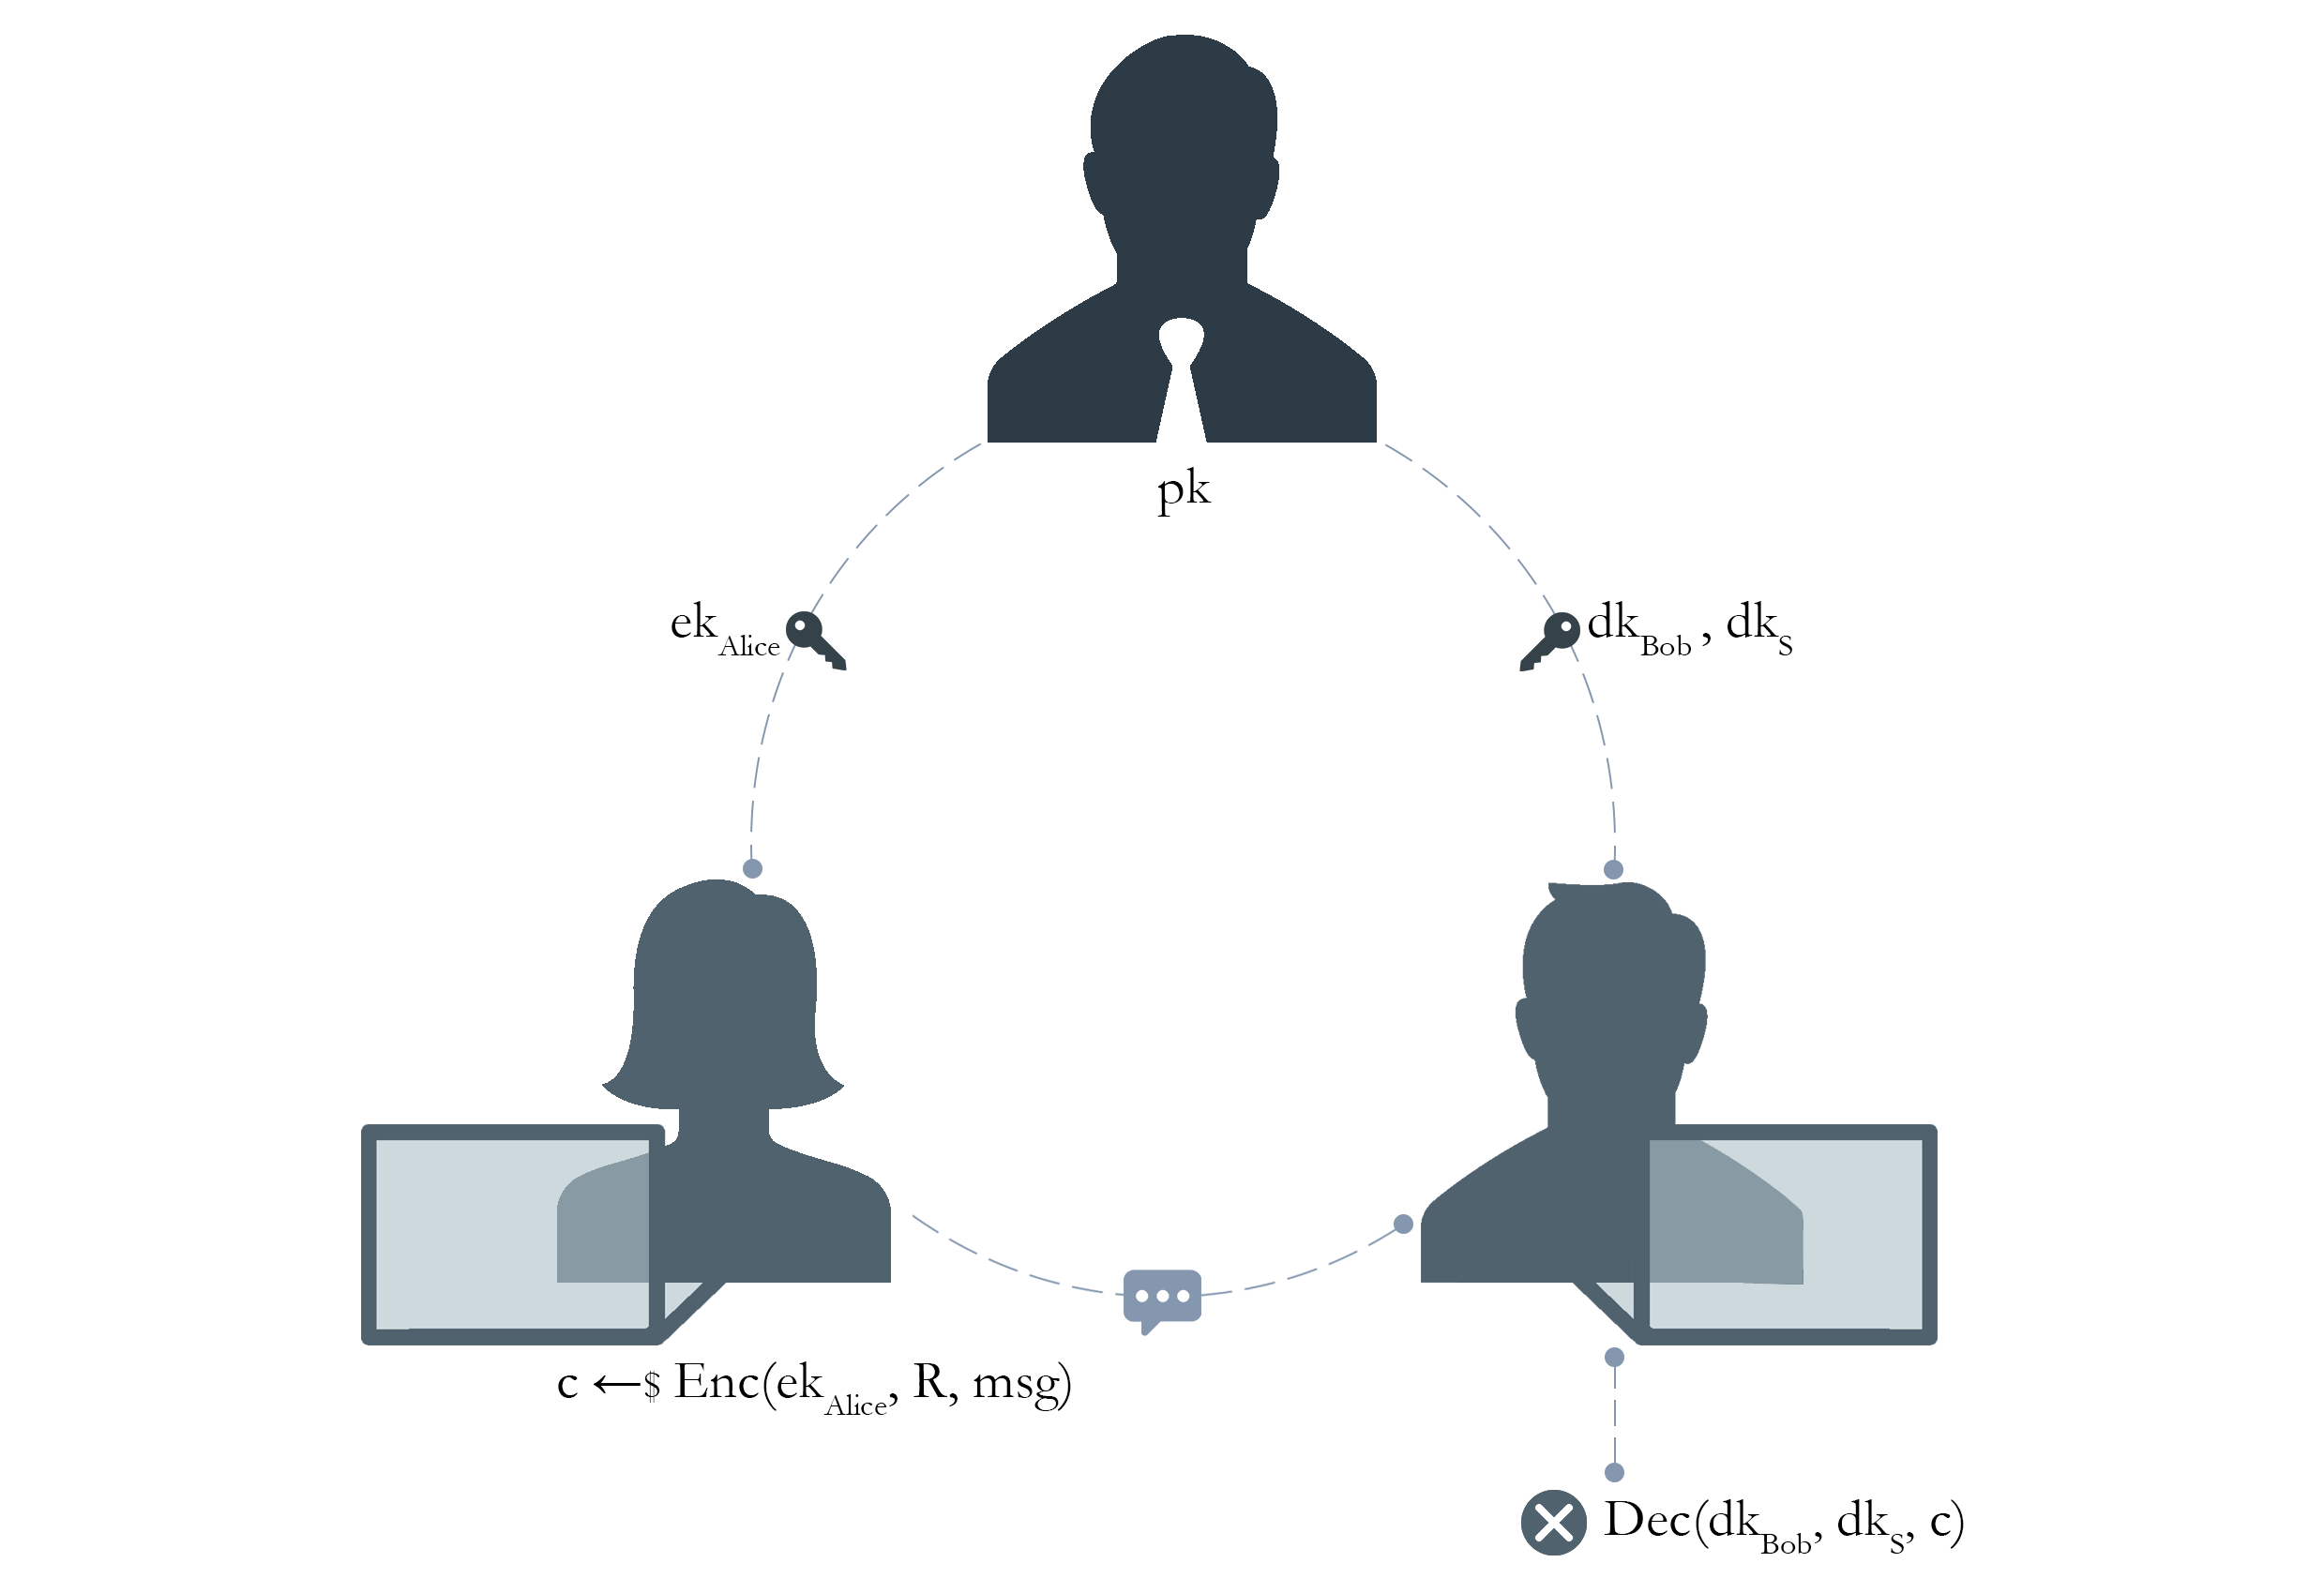
\includegraphics[width=\linewidth]{images/me.png}
    \caption{ME example. Alice encrypts a message with her encyrption key $\ek_{Alice}$, provided by the trusted party: she specifies some arbitrary policy $\raccess$. When Bob receives the ciphertext, tries to decrypt it with his decryption key $\dk_{Bob}$ and a key associated with some arbitrary policy $\saccess$.}
    \label{fig:me_example}
\end{figure}
\newline\newline
Matchmaking Encryption can be thought of as a non-interactive version of Secret Handshakes (see \ref{sec:sh}), introduced in 2003 by Balfanz et al. \cite{Balfanz}.
Indeed, ME gives privacy guarantees similar to that of SH, but it provides a more efficient way to communicate (being non-interactive) and, at the same time, it is more flexible since a party is not constrained to a group.

\section{Security}
Security is defined via two properties: privacy and authenticity.

\paragraph{Privacy}
Intuitively, privacy aims at capturing secrecy of the sender’s inputs in presence of malicious receivers: during the decryption nothing is leaked beyond the fact that a match occurred or did not occur; in particular, in case of mismatch, the reason why the match did not occur is not revealed.
This is a much stronger guarantee w.r.t the one addressed by dual policy ABE schemes,\footnote{Here the sender encrypts a message by choosing both a policy and a set of attributes; the receiver can decrypt the ciphertext using a decryption key associated to both the receiver’s policy and attributes.} introduced by Attrapadung and Imai \cite{Attrapadung}, which only protects the secrecy of the message.
In order to ensure such a guarantee, any ME construction needs to face the technical challenge of simultaneously checking the policies chosen by S and R: this check can be seen as an atomic operation.

\paragraph{Authenticity}
Authenticity, on the contrary, captures security against malicious senders: more formally, it demands that the only way to produce a valid ciphertext under attributes $\sigma$ is to obtain an encryption key corresponding to $\sigma$ from the authority, thus guaranteeing that if a ciphertext decrypts correctly, then it has been created by a sender with the proper encryption key.

\section{Arranged ME}
Ateniese et al. also defined a possible variant of ME, namely Arranged Matchmaking Encryption (A-ME).
The main difference is that in A-ME there is a single decryption key $\dk_{\rattr,\saccess}$ which describes simultaneously the receiver's
attributes $\rattr$ and the policy $\saccess$ chosen by the receiver, while ME makes use of two different keys: one for the policy and the other one for the receiver's attributes.

\section{Thesis contributions}
\paragraph{CCA security}
In this document, we revamp the notion of ME by extending the security definitions to the setting of chosen-ciphertext attacks (CCA).
In this context ciphertexts cannot be malleable\footnote{If malleable, given an encryption of a message m, it is possible to generate another ciphertext which decrypts to f(m), for some function f, without necessarily knowing or learning m.} anymore.
\newline\newline
We define these two new properties:
\begin{itemize}
    \item CCA-privacy: the adversary may now additionally have access to a decryption oracle that answers decryption queries. This captures privacy even in the presence of attackers that can obtain the decryption of possibly mauled ciphertexts. See \ref{sec:cca-privacy}.
    \item CCA-authenticity: the attacker is also given access to an encryption oracle. This captures authenticity in the presence of attackers that try to generate valid ciphertexts by mauling previously obtained ciphertexts. See \ref{sec:cca-auth}.
\end{itemize}
We studied CCA security both for ME and A-ME, in order to capture stronger security guarantees w.r.t. the chosen-plaintext attack (CPA) scenario, addressed in the original paper.
Indeed, CCA security is of seminal importance in many practical situations: e.g. in 1998 Bleichenbacher showed how to crack an SSL session key in less than a day, simply sending several ciphertexts to a decryption device \cite{Bleichenbacher}.

\paragraph{Constructions}
We finally define black-box constructions to transform any CPA-secure ME (resp. A-ME) scheme into a CCA-private ME (resp. A-ME) scheme, by relying on a Non-Interactive Zero-Knowledge (NIZK) argument system and a Signatures scheme.
\newline\newline
In our construction (see \ref{sec:cca-transformation}), to encrypt message $m$ under sender attributes $\sigma$ and policy $\mathbb{R}$ we proceed as follows: we first encrypt $m$ using the underlying ME (resp. A-ME) scheme; then we add a NIZK argument of the knowledge of the plaintext $m$ and a valid signature $s$ on $\sigma$, where the signature is provided by a trusted party.
\newline
We prove that these two constructions achieve CCA-privacy and preserve the authenticity of the underlying schemes.
